To design the feedback controller $u_e(k) = \kappa (\text{x}(k),x_{ref}(k))$, we want to choose the closed loop eigenvalues by means of the \textit{Arbitrary Eigenvalue Assignment}. 
According to the control requirement, the frequency band is [20,\ 200] Hz. The eigenvalues were then selected to have a sharp control between these bounds. To do so, the natural frequency $w_n$ was chosen to be more than $2\pi \cdot 200 = 1.26 \cdot 10^3 \ rad/sec$. We also wanted a good damping ratio, around 0.7 as well as a fast time constant. Finally the eigenvalues need to have a negative real part to get a stable system. These criteria were fulfilled but for 200 Hz, the tracking was unsactisfactory. The eigenvalues were increased little by little to find the best trade-off between the control input which has to be in the range -40 and 40 V and and a suitable tracking. It was finally chosen to multiply the eigenvalues obtained with the criteria above by $1.4$. Converted in discrete time thanks to the formula $\lambda_F = e^{\lambda_A Ts}$, the desired eigenvalues are:

\begin{equation*}
\lambda_{Fdesired} =  \begin{pmatrix}
0.3263\\
0.6868 - 0.1975i\\
0.6868 + 0.1975i
\end{pmatrix}
\end{equation*}

As it is explained in P14, the controller to be implemented is a reference feedforward. We have $u_e(k) = -K\text{x}(k) + Nx_{ref}(k)$, where $K$ and $N$ are gains that we need to determine.
The feedback gain K is computed thanks to the Ackermann's formula in Matlab $K = acker(F,G,\lambda_{Fdesired})$ and we obtain our new system with $F_k = F-GK$. The good placement of the eigenvalues is checked thanks to the \textit{eig} function. The bode diagram is also plotted (figure \ref{fig:bodeLambda}) and it can be verified that the gain is constant for the frequency band desired from 20 to 200 Hz i.e. from $126$ rad/sec to $1.26 \cdot 10^3$ rad/sec. 

\begin{figure}[H]
 \centering 
 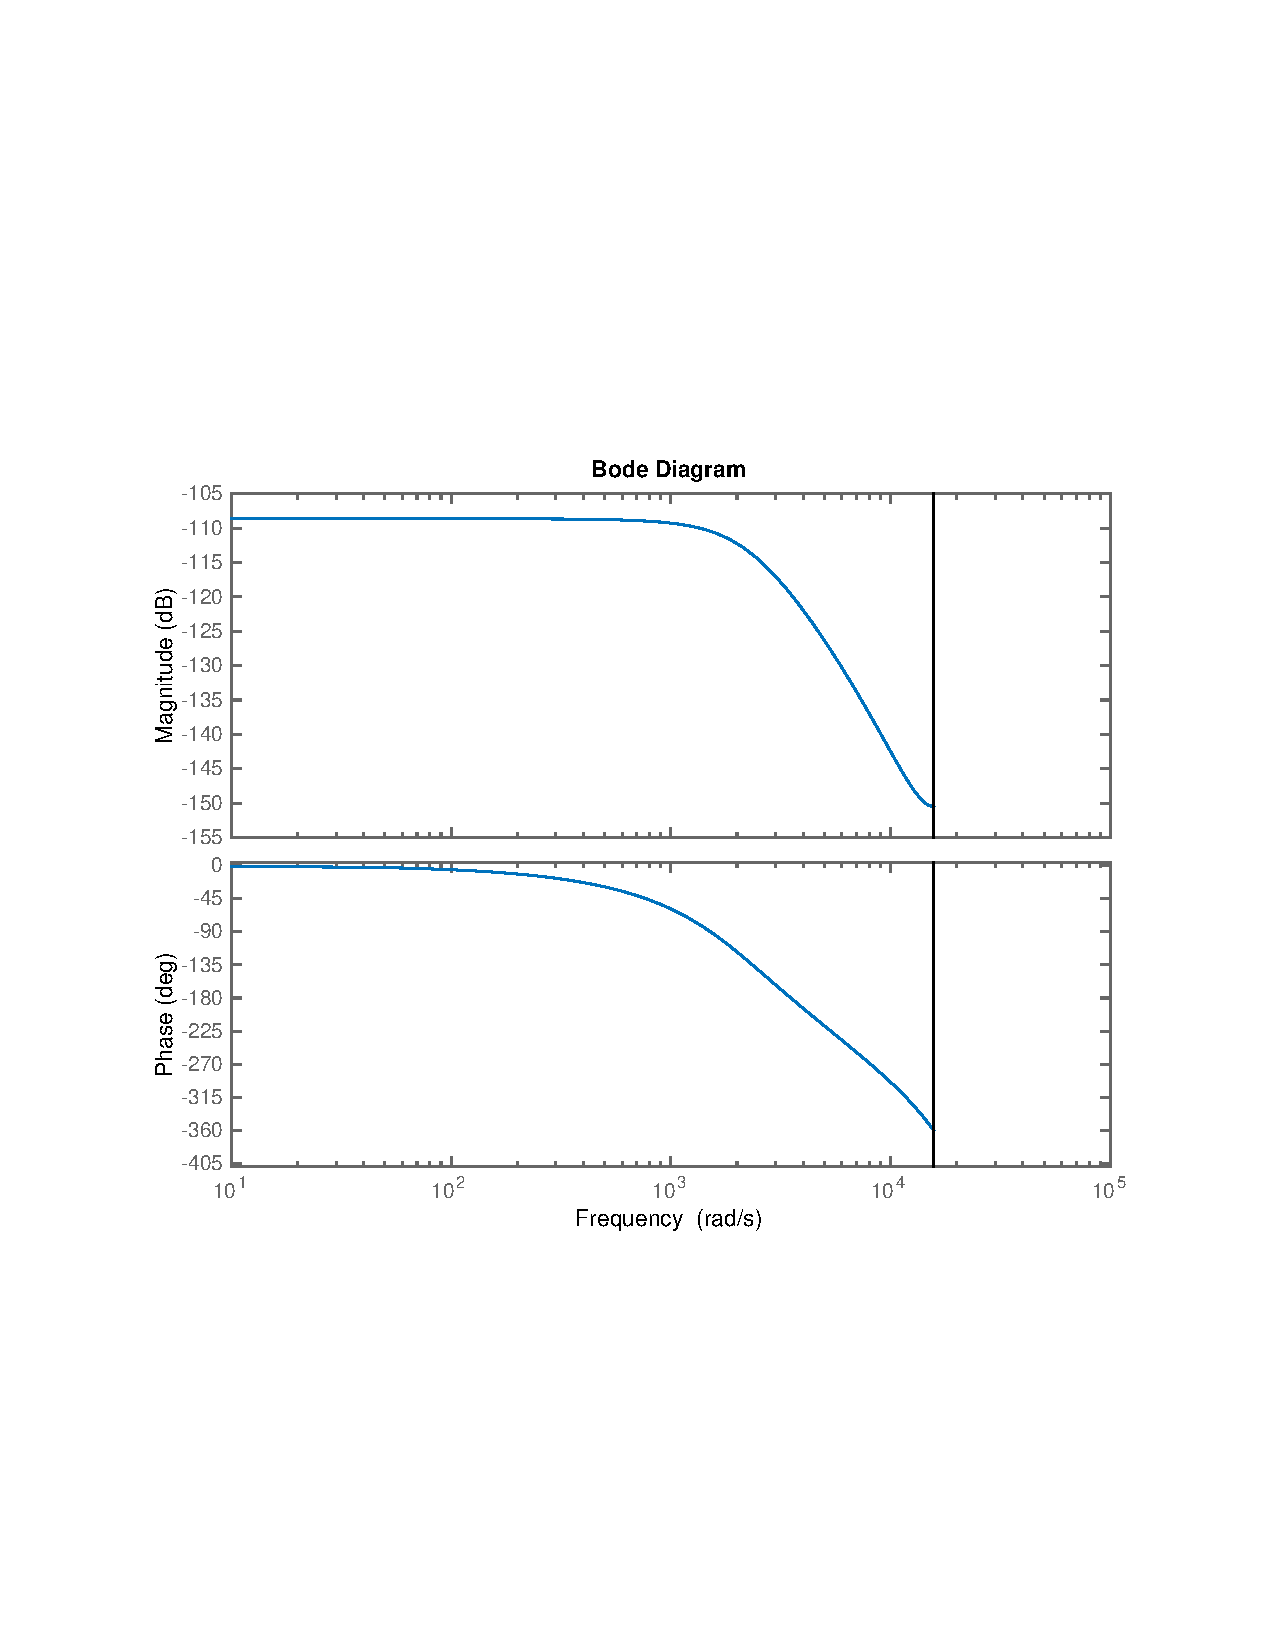
\includegraphics[trim=2cm 7cm 2cm 7cm, clip=true, totalheight=0.35\textheight, angle=0]{figures/P15bodeLambda.pdf}
 \caption{Bode Diagram of the Discrete Time System with Feedback Controller}
 \label{fig:bodeLambda}
\end{figure}

Once this step achieved, we compute $N$ \eqref{gainN} through the DC gain $\kappa$ of the closed-loop system \eqref{DCgain}:
\begin{align}
\kappa &= C(I-F_k)^{-1}G \label{DCgain} \\
N &= \kappa^{-1} \label{gainN}
\end{align}

After implementing the controller in Simulink (see Appendix \ref{AppDiscreteTimeP15}), the simulation was run. It can be noticed on figure \ref{fig:P15xref} that the voice coil position matches well the reference $x_{ref}$ with a time delay $\tau = 1 \ ms$.
\begin{figure}[H]
 \centering 
 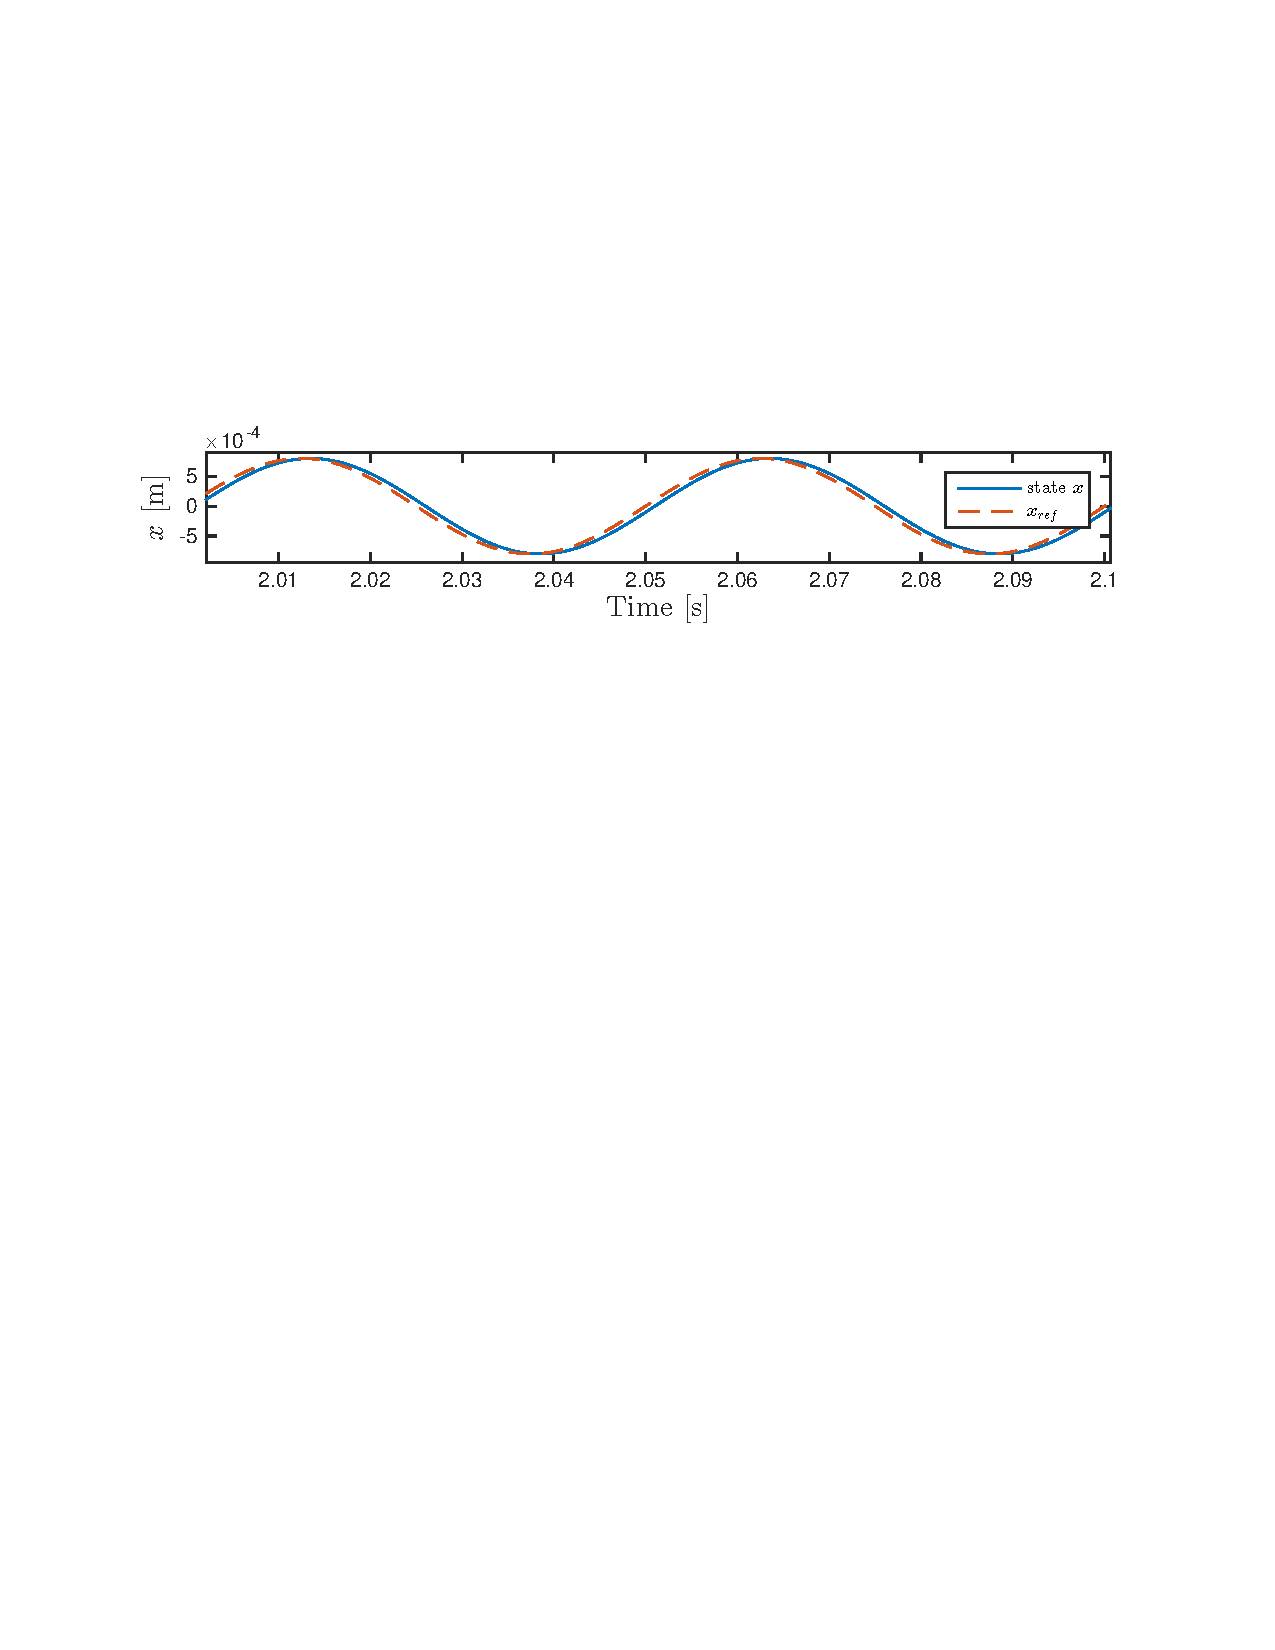
\includegraphics[trim=2cm 17cm 2cm 7cm, clip=true, totalheight=0.12\textheight, angle=0]{figures/P15xref.pdf}
 \caption{Simulation of the Discrete Time Linear Model with the Position Reference Tracking}
 \label{fig:P15xref}
\end{figure}